\documentclass{article}

\usepackage{microtype}
\usepackage{graphicx}
\usepackage{booktabs} % for professional tables
\usepackage{caption}
\usepackage{subcaption} % for subcaption boxes
\usepackage{amsmath}
\usepackage{bm}      % for bold greek letters
\usepackage{amssymb} % more math symbols
\usepackage{amsthm}
\usepackage{bbm}  % blackboard 1
\usepackage{hyperref}
\usepackage{paralist}
\usepackage{wrapfig}
\newcommand{\theHalgorithm}{\arabic{algorithm}}
\usepackage{comment}

\PassOptionsToPackage{sort, numbers, compress}{natbib}

\usepackage[preprint]{neurips_2020}
\setcitestyle{square}

\renewcommand{\subsubsection}[1]{\textbf{#1}

} % newlines are deliberate
\DeclareMathOperator*{\argmax}{arg\,max}
\DeclareMathOperator*{\argmin}{arg\,min}
\DeclareMathOperator*{\E}{\mathbb{E}}
\newcommand{\reals}{\mathbb{R}}
\newcommand{\naturals}{\mathbb{N}}
\newcommand{\sig}{\mathrm{Sig}^N}
\newcommand{\dataspace}{\mathcal{X}}
\newcommand{\lspace}{\mathcal{Y}}
\newcommand{\seriesspace}{\mathcal{S}}
\newtheorem{theorem}{Theorem}
\newcommand{\data}[1]{\mbox{\textsc{#1}}}   % can be used to typeset arbitrary data set set names

\title{Path Imputation Strategies for Signature Models}
% Alternative Title:
%% Path Imputation Strategies with Signature Models for Irregularly Sampled Partially Observed Multivariate Time Series.

\author{
    Michael Moor$^1$
    \And
	Patrick Kidger$^{2, 3}$
	\And
	Max Horn$^1$
	\And
	Christian Bock$^1$
	\And
	Bastian Rieck$^1$
	\And
	Karsten Borgwardt$^1$
	\AND \\[-12pt]
	\null$^1$ Department of Biosystems Science and Engineering, ETH Zurich
	\\
	\null$^2$ Mathematical Institute, University of Oxford \\
	\null$^3$ The Alan Turing Institute, British Library
	\\
	\hspace{-6.5em}\texttt{\{michael.moor, max.horn, christian.bock,}
	\\
	\hspace{6.5em}\texttt{bastian.rieck, karsten.borgwardt\}@\hspace{0.1pt}bsse.ethz.ch}
	\\
	\texttt{kidger@\hspace{0.1pt}maths.ox.ac.uk}
} % TODO: are the emails I've guessed correct?

\begin{document}
\maketitle

\begin{abstract}
The signature transform is a `universal nonlinearity' on the space of continuous vector-valued paths, and has recently received attention for use in machine learning. However real-world temporal data is typically discretized, and must first be transformed into a continuous path before signature techniques can be applied. %, which has previously been described as an embedding problem. 
Our first contribution is to characterise this as an imputation problem, and to empirically assess the impact of various imputation techniques when applying the signature to irregular time series data. Throughout our experiments, we observe that uncertainty-aware \emph{predictions} are beneficial, even compared to the uncertainty-aware \emph{training} of Gaussian process (GP) adapters. We thus also propose a simple extension of GP adapters by integrating uncertainty to the prediction step which leads to competitive performance.
\end{abstract} % TODO: touch this up a bit, but I think the essential idea is there.

% % Suggestion (BR):
% \begin{abstract}
% The signature transform, a `universal non-linearity' on the space of
% continuous vector-valued paths, recently started receiving attention in
% machine learning applications. Prior to applying any signature technique,
% real-world temporal data is typically discretised and
% subsequently transformed into a continuous path. While this is commonly
% treated as an embedding problem, we characterise it as an
% \emph{imputation problem} instead, and empirically assess the impact of
% numerous imputation techniques on the classification of
% irregularly-sampled time series data sets by means of signature
% techniques. We observe throughout our experiments that uncertainty-aware
% \emph{predictions} are beneficial, even compared to the
% uncertainty-aware \emph{training} of Gaussian Process~(GP) adapters. We
% thus also propose a simple extension to the prediction step of GP
% adapters and demonstrate that it leads to competitive performance.
% \end{abstract}

% %OLD VERSION:
% \section{Introduction}\label{intro}
% Originally described in \cite{Chen54, Chen57, Chen58} and popularised in the theory of rough paths and controlled differential equations \cite{lyons1998differential, FritzVictoir10, lyons2014rough}, the \emph{signature transform}, also known as the \emph{path signature} or simply \emph{signature}, acts on a continuous vector-valued path of bounded variation, and returns a graded sequence of statistics, which determine the path up to a negligible equivalence class.

% Every continuous function of a path can be recovered by applying a linear transform to this collection of statistics \cite[Proposition A.6]{kidger2019deep}. This `universal nonlinearity' property makes the signature a promising nonparametric feature extractor.

% Given their similarities, it is natural to hope that the tools that apply to continuous paths may also be applied to multivariate time series. Of course, multivariate time series are not continuous paths. For signature techniques to be applied, a continuous path must first be constructed from this data.

% In previous work \cite{kidger2019deep, levin2013, fermanian2019embedding} this has been characterised as an embedding problem, and has typically been glossed over as an essentially unimportant detail. This is exacerbated by the (perfectly sensible) behaviour of software for computing the signature \cite{iisignature, signatory}, which take a continuous piecewise linear path as an input, described by its sequence of knots. This resembles a sequence of data, meaning that the signature is sometimes interpreted as operating on sequences of data rather than on paths \cite{kidger2019deep, levin2013}.

% \subsection{Contributions}
% In this paper we reinterpret of the task of constructing a continuous path, by turning it from an embedding problem into an imputation problem. To distinguish this from traditional imputation problems, we refer to this as \emph{path imputation}.

% Much previous literature on the signature transform has focused on its excellent theoretical properties, in particular sampling independence \cite[Proposition A.7]{kidger2019deep}, \cite{signatorydocumentation}, \cite[Section 2]{toth2019gp}, but our findings show that this does not correspond to empirical performance. However it has previously been established that observation rates and missingness itself can carry information \cite{rubin1976inference, gelman2007dataanalysis}. By re-interpreting the task of constructing paths as an imputation problem, we identify that this performance gap is likely to be another manifestation of this phenomenon.

% We perform a thorough empirical investigation of various imputation schemes as combined with multiple models that potentially employ signatures. We find that approaches that have access to uncertainty information \emph{during prediction} tend to outperform the competitors, also uncertainty-aware frameworks where the uncertainty is only available during \emph{training}, such as Gaussian process (GP) adapters.
% Motivated by this, we propose a novel extension of GP adapters \cite{li2016scalable, futoma2017mgp} which incorporates uncertainty information into the prediction step, which helps our task at hand but could also be of independent interest.
% As a footnote we observe that the recently introduced `deep signature models' \cite{kidger2019deep} consistently outperform other signature models, which also suffer from much higher variance in their efficacy.

% Our code is available at XXXXXX.

%%%%%%%%%%%%%%%%%%%%%%%%%%%%%%%%%%%%%%%%%%%%%%%%%%%%%%%%%%%%%%%%%%%%%%%%
% Introduction (suggestion, BR) 
%%%%%%%%%%%%%%%%%%%%%%%%%%%%%%%%%%%%%%%%%%%%%%%%%%%%%%%%%%%%%%%%%%%%%%%%

\section{Introduction}

Originally described by \citet{Chen54, Chen57, Chen58} and popularised
in the theory of rough paths and controlled differential
equations~\cite{lyons1998differential, FritzVictoir10, lyons2014rough},
the \emph{signature transform}, also known as the \emph{path signature}
or simply \emph{signature}, acts on a continuous vector-valued path of
bounded variation, and returns a graded sequence of statistics, which
determine a path up to a negligible equivalence class. Moreover,
it can be shown~\cite[Proposition A.6]{kidger2019deep} that \emph{every}
continuous function of a path can be recovered by applying a linear
transform to this collection of statistics. This `universal
nonlinearity' property makes the signature a promising nonparametric
feature extractor with beneficial properties in both generative and
% TODO: consider adding more citations here
supervised learning scenarios~\citep{kidger2019deep}.
%
Given their similarities, it is natural to hope that the tools that
apply to continuous paths may \emph{also} be applied to multivariate
time series. Of course, multivariate time series are not continuous
paths---in fact, for signature techniques to be applied, one first needs
to construct a continuous path from this kind of data.

In previous work~\cite{kidger2019deep, levin2013, fermanian2019embedding}, this
construction has been characterised as an embedding problem, and was
typically glossed over as a rather unimportant detail.
%
This is exacerbated by the---perfectly sensible---behaviour of software
for computing the signature \cite{iisignature, signatory}, which
commonly considers a continuous piecewise linear path as an input,
% TODO: is there a better definition of 'knot'? I am aware of the
% meaning in terms of spline approximations, but maybe we could clarify
% this here.
described by its sequence of knots, i.e.\ values.
%
Since such sequences resemble a sequence of data, the signature is
sometimes interpreted as operating on sequences of data rather than on
paths~\cite{kidger2019deep, levin2013}.
%
We show that this view is somewhat limiting and that, in order to
achieve competitive predictive performance for real-world time series
classification, it is crucial to consider the path construction process.

Specifically, in this paper we reinterpret the task of
constructing a continuous path, by turning it from an embedding problem
into an imputation problem. To distinguish this from traditional
imputation problems, we refer to this as \emph{path imputation}.
%
While a large part of the previous literature on the signature transform
focused on its excellent theoretical properties, in particular sampling
independence~\cite[Proposition A.7]{kidger2019deep},~\cite{signatorydocumentation},~\cite[Section 2]{toth2019gp}, our findings show that this does not
necessarily correspond to excellent empirical performance.
%
However, it has previously been established that both observation rates
and missingness itself can carry information in time series
classification tasks~\citep{rubin1976inference, gelman2007dataanalysis}.
%
Our reinterpreted view of path construction as an imputation problem
permits us to identify that this performance gap is likely another
manifestation of the phenomenon of glossing over imputation details.

We therefore perform a thorough empirical investigation of various
imputation schemes in combination with multiple models that can potentially
employ signatures. We find that approaches that have access to
uncertainty information \emph{during prediction} tend to outperform the
competitors, even uncertainty-aware frameworks for which this
information is only available during \emph{training}, such as Gaussian
Process~(GP) adapters~\citep{li2016scalable, futoma2017mgp}.
%
Motivated by this, we propose a novel extension of GP adapters that
directly incorporates uncertainty information into the prediction step,
thus improving predictive performance.
Throughout our experiments, we observe that the recently introduced
\emph{deep signature models}~\citep{kidger2019deep} consistently
outperform other signature models~(which in turn suffer from increased
variance, thus reducing their efficay).
%
We make our code publicly available under XXXXXX.

%%%%%%%%%%%%%%%%%%%%%%%%%%%%%%%%%%%%%%%%%%%%%%%%%%%%%%%%%%%%%%%%%%%%%%%%
% Old content starts here
%%%%%%%%%%%%%%%%%%%%%%%%%%%%%%%%%%%%%%%%%%%%%%%%%%%%%%%%%%%%%%%%%%%%%%%%

\section{Related work}

A key motivation for this work is the use of the signature transform in
machine learning: in recent work~\citep{primer2016,
kormilitzlin2016, yang2016rotation, li2017lpsnet, yang2017leveraging,
PerezArribas2018, morrill2019sepsis} the signature transform is
typically used as a nonparametric feature extractor, on top of which
a model is learnt. A growing body of work has also investigated how to
integrate the signature transform more tightly with neural networks; 
\citet{jeremythesis}, \citet{logsigrnn}, and \citet{kidger2019deep} all
study how to use the signature transform\footnote{And the related
logsignature transform; the difference between them will not be
important for us.} within typical neural network models.
\citet{chevyrev2018signature, kiraly2019kernels} study how the signature
transform may be used to define a \emph{kernel}---i.e.\ a symmetric,
positive definite function that is typically used as a similarity
measure---on path space, while \citet{toth2019gp} show how this kernel
may be used to define a Gaussian process.

In much of this work, data has been converted into a continuous path via
linear interpolation. Some authors~\citep{primer2016,
fermanian2019embedding} have additionally considered `rectilinear'
interpolation, which is similar. \citet{levin2013} present the
`time-joined transformation', which is a hybrid of the two, such that
the resulting path exhibits a causal dependence on the data.  However,
to our knowledge, no prior work has regarded this as an imputation
problem.

The general problem of imputing data is well-known and well-studied, and
we will not attempt to describe it here; see for example \citet[Chapter 25]{gelman2007dataanalysis}.
% Common simple imputation schemes are to impute missing values as the mean of its channel, or to forward fill the last observed value, although it has been observed that incautious use of such methods can result in heavily biased models \cite{Molnar2008}.
These methods typically only fill in missing discrete data points, and do not attempt to impute the underlying continuous path.
%
One approach that does impute a \emph{full} continuous path is
a Gaussian process adapter~\citep{li2016scalable, futoma2017mgp}. The
data is modelled as coming from a Gaussian process. The posterior
distribution, having observed the data, then gives continuous paths
through data space. This then allows, for example, for uniformly
resampling the data. Gaussian process adapters will be important to this
study, although in our case they are of interest not because of uniform
resampling, but because they provide a full continuous path, which we may
sample arbitrarily. We note that there are also other approaches that
perform continuous-time imputation~\citep{shukla2018interpolationprediction},
but we have not investigated these further.

%%%%%%%%%%%%%%%%%%%%%%%%%%%%%%%%%%%%%%%%%%%%%%%%%%%%%%%%%%%%%%%%%%%%%%%%
\section{Background}
%%%%%%%%%%%%%%%%%%%%%%%%%%%%%%%%%%%%%%%%%%%%%%%%%%%%%%%%%%%%%%%%%%%%%%%%

% TODO: can we summarise what we are doing here? What are the most
% important points of this section?
%
% Maybe: 'In the following, we provide a cursory introduction to the
% path signature methods. Please refer to XXX for a more in-depth
% description.'

\subsection{Path signatures}

Given a continuous, piecewise differentiable path $f \colon [a, b] \to
\reals^d$, the \emph{signature transform up to depth $N$} may be defined
by
%
\begin{equation}
    \sig(f)=\left(\left(\underset{\,a<t_{1}<\cdots<t_{k}<b}{\int \cdots \int} \prod_{j=1}^{k} \frac{\mathrm{d} f_{i_{j}}}{\mathrm{d} t}\left(t_{j}\right) \mathrm{d} t_{1} \cdots \mathrm{d} t_{k}\right)_{1 \leq i_{1}, \ldots, i_{k} \leq d}\right)_{1 \leq k \leq N}.
\end{equation}

% \begin{wrapfigure}{l}{4cm}
%     \centering
%     \vspace{-2em}
% 	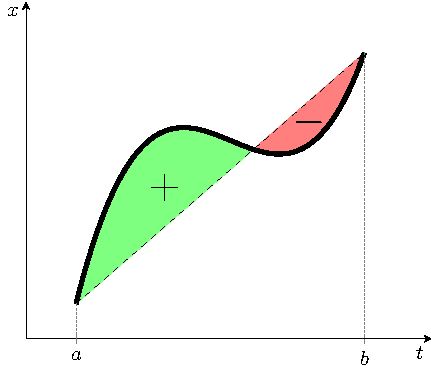
\includegraphics[width=0.3\columnwidth]{figures/sig_path1.pdf}
% 	\caption{Given a path, shown in bold, its Levy area is its signed area with respect to the chord joining its endpoints.}\label{fig:sig_path}
% 	\vspace{-2em}
% \end{wrapfigure}

%This definition may be extended to paths of merely bounded variation by replacing these integrals with Riemann--Stieltjes integrals, and extended further to paths of bounded $p$-variation by replacing them with rough integrals \cite{lyons1998differential}.

In brief, the signature transform may be interpreted as extracting
information about \emph{order} and \emph{area} of a path.
%
One may interpret its terms as `the area/order of one channel with
respect to some collection of other channels'.
%
% As an explicit example of the sort of information extracted, one of the things computed by the signature is the \emph{Levy area} of the path, shown for a one-dimensional example in Figure \ref{fig:sig_path}.
%
For an exposition on the properties of the signature transform and its
use in machine learning, please refer to \citet{primer2016} or \citet[Appendix A]{kidger2019deep}.
%
%There is one fact that will prove important to our arguments later, however, so for completeness we repeat it here:
%\begin{theorem}[Invariance to reparameterisation]\label{theorem:invariancetime}
%Let $f \colon [a, b] \to \reals^d$ be a continuous piecewise differentiable path. Let $\psi \colon [a, b] \to [c, d]$ be continuously differentiable, increasing, and surjective. Then $\sig(f) = \sig(f \circ \psi)$.
%\end{theorem}

%\subsubsection{Comparison to the Fourier and wavelet transforms}
%The signature transform exhibits a certain similarity to the one-dimensional Fourier or wavelet transforms. Both are integrals of paths. However, in reality these transforms are fundamentally different. Both the Fourier and wavelet transforms are linear transforms, and operate on each channel of the input path separately. In doing so they model the path as a linear combination of elements from some basis.
%
%Conversely, the signature transform is a nonlinear transform - indeed, it is a universal nonlinearity - and operates by combining information between different channels of the input path. In doing, the signature transform models \emph{functions of the path}; the universal nonlinearity property says that in some sense it provides a basis for such functions.

%\subsubsection{Computing the signature transform}
%Continuous piecewise linear paths are the paths of choice, computationally speaking, due to the fact that this is the only case for which efficient algorithms for computing the signature transform are known \cite{signatory}.
%
%This is not a serious hurdle when one wishes to compute the signature of a path $f$ that is not piecewise linear -- as the signature of piecewise linear approximations to $f$ will tend towards the signature of $f$ as the quality of the approximation increases -- but it does enforce this requirement on our imputation schemes.
%
%Thus all of the imputation schemes we examine will first seek to select a collection of points in data space (not necessarily only where we had data before), and then linear imputation will be performed to join them up into a piecewise linear path.

%%%%%%%%%%%%%%%%%%%%%%%%%%%%%%%%%%%%%%%%%%%%%%%%%%%%%%%%%%%%%%%%%%%%%%%%
\subsection{Notation}
%%%%%%%%%%%%%%%%%%%%%%%%%%%%%%%%%%%%%%%%%%%%%%%%%%%%%%%%%%%%%%%%%%%%%%%%

Given some set $A$, let the space of time series over $A$ be defined by
\begin{equation}
    \seriesspace(A) = \{((t_1, x_1), \ldots, (t_n, x_n)) \,\vert\, t_i \in \reals, x_i \in A, n \in \naturals, \text{ such that } t_1 \leq \cdots \leq t_n\}.\label{eq:seriesspace}
\end{equation}
%
Note the subtle point that the $t_i$ are separated by $\leq$, not $<$.
We make this slight change because it will later prove important for one
of our studied imputation schemes. For example, contrast the
corresponding definition in \citet[Section 1]{toth2019gp}.

\paragraph{Time series and labels.}
%
Let $\lspace$ be a set and let $\dataspace_j = \reals$ for $j \in \{1,
\ldots, d\}$ and $d \in \naturals$. Then we assume that we observe
a dataset of labelled time series $(\mathbf{x}_k, y_k)$ for $k \in \{1,
\ldots, N\}$, where $\mathbf{x}_k \in \seriesspace(\dataspace^*)$ and
$y_k \in \lspace$, with $\dataspace^* = \prod_{j = 1}^d(\dataspace_j
\cup \{*\})$ and $*$ representing no observation.
%
We similarly define $\dataspace = \prod_{j = 1}^d\dataspace_j$. Thus,
$\dataspace$ is the data space, while $\dataspace^*$ is the data space
allowing missing data, and $\lspace$ is the set of labels.

% \subsubsection{Terminology for imputation schemes}
% To avoid ambiguity, we will refer to standard imputation schemes, such as forward-fill, as a \emph{data-imputation} scheme, meaning to impute missing data points. In contrast we will use \emph{path-imputation} to describe the more general task of imputing the full continuous path.

\subsection{Gaussian process adapter}\label{section:gpadapter}

Some~(but not all) of the imputation schemes we consider are based on
the uncertainty aware-framework of multi-task Gaussian process
adapters~\citep{li2016scalable, futoma2017mgp}.
%
Let $\mathcal{W}, \mathcal{H}$ be some sets. Let $\ell \colon \lspace
\times \lspace \to [0, \infty)$ be a loss function. Let $F \colon
\dataspace^{[a, b]} \times \mathcal{W} \to \lspace$, be some (typically
neural network) model, with $\mathcal{W}$ interpreted as a space of
parameters. Let \begin{align*} \mu \colon [a, b] \times
\seriesspace(\dataspace^*) \times \mathcal{H} &\to \dataspace\\ \Sigma
\colon [a, b] \times [a, b] \times \seriesspace(\dataspace^*) \times
\mathcal{H} &\to \dataspace    \end{align*} be mean and covariance
functions, with $\mathcal{H}$ interpreted as a space of
hyperparameters. The dependence on $\seriesspace(\dataspace^*)$ is to
represent conditioning on observed values.

Then the goal is to solve
\begin{equation}\label{eq:gp-mc}
\argmin_{\mathbf{w} \in \mathcal{W},\bm{\eta} \in \mathcal{H}} \sum_{k=1}^N \overbrace{\rule{0pt}{0.5cm} \mathbb{E}_{\mathbf{z}_k \sim \mathcal{N}\left( \mu(\cdot, \mathbf{x}_k, \eta), \Sigma(\cdot, \cdot, \mathbf{x}_k, \eta)\right) } \big[ \ell(F(\mathbf{z}_k, \mathbf{w}),
y_k) \big] }^{\text{$E_k$}}.
\end{equation}
%
As this expectation is typically not tractable, it is estimated by Monte
Carlo (MC) sampling with $S$ samples, i.e.\
\begin{equation}
E_k \approx \frac{1}{S} \sum_{s=1}^{S} \ell(F(\mathbf{z}_{s, k}, \mathbf{w}), y_k),
\end{equation}
%
where
%
\begin{equation}
    \mathbf{z}_{s, k} \sim \mathcal{N}\left( \mu(\,\cdot\,, \mathbf{x}_k, \eta), \Sigma(\,\cdot\,, \,\cdot\,, \mathbf{x}_k, \eta)\right).
\end{equation}

Alternatively, one may forgo allowing the uncertainty to propagate through $F$ by instead passing the posterior mean directly to $F$; this corresponds to solving
\begin{equation}\label{eq:gp-mean}
\argmin_{\mathbf{w} \in \mathcal{W},\bm{\eta} \in \mathcal{H}} \sum_{k=1}^N \ell(F(\mu(\,\cdot\,,\mathbf{x}_k, \eta), \mathbf{w}), y_k).
\end{equation}


\begin{comment}
\subsubsection{Application beyond signatures}

Whilst the task of converting observed data into a path in data space is particularly important for signatures, it also arises in the context of, for example, convolutional and recurrent neural networks.

Convolutions are often thought of in terms of discrete sums, but they are perhaps more naturally described as the integral cross-correlation between the underlying data path $f$ and the learnt filter $g_\theta$. Given sample points $t_1, \ldots, t_n \in [0, T]$, this integral is then approximated via numerical quadrature:
\begin{equation*}
    \frac{1}{T}\int_0^T f(t) g_\theta(t) \mathrm{d}t \approx \frac{1}{n}\sum_{i = 1}^n f(t_i) g_\theta(t_i),
\end{equation*}
although the $1/n$ scaling is really only justified in the case that the $t_i$ are equally spaced.\footnote{The $g_\theta$ is typically a step function in `normal' convolutional layers. Some works exists on replacing it with e.g. B-splines \cite{fey2018splinecnn} to better handle irregular data. The oddity of scaling by $1/n$ with irregular data has not been explicitly addressed in the literature, at least to our knowledge; indeed quite conversely we have seen it used without remark.} Thus we see that with convolutions, we are implicitly interpreting the observed data as a path in data space.

Similarly, the connection between dynamical systems and recurrent neural networks are well known \cite{FUNAHASHI1993801, continuousrnn}, and these tend to use a similar setup.

For non-signature methods as for signature methods, this implicit usage of data as a path in data space often seems to be swept under the rug, and we suspect it is one deserving further attention. However our focus here is specifically on solutions appropriate for signatures, and this larger problem is not one that we will explore further in this paper.
\end{comment}

\begin{figure}[t]
    \centering
    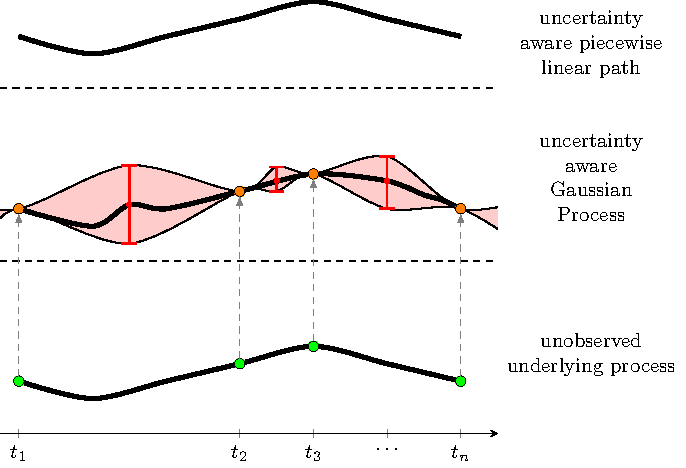
\includegraphics{figures/overview.pdf}
    \caption{Overview of our proposed extension of GP adapters, GP-PoM, leveraging both posterior moments (mean and variance)}
    \label{fig:overview}
\end{figure}


\section{Path imputations}
%For simplicity of presentation, we will now assume that $\dataspace_j = \reals$.%, although in principle the theory actually only requires that $\dataspace_j$ is a Banach space.

Our goal is to learn a function from $\seriesspace(\dataspace^*)$ to
$\lspace$. Motivated by signature theory, we believe that this is best
done by selecting a path imputation strategy
% Our belief (perhaps merely motivated by signature theory, but in this paper explicitly because we wish to apply signatures), is that this is sensibly done by selecting a path-imputation strategy
%
\begin{equation}
    \phi \colon \seriesspace(\dataspace^*) \to (\reals \times \dataspace)^{[a, b]},
\end{equation}
and only \emph{afterwards} learning a map from $\dataspace^{[a, b]}$ to $\lspace$.
%
Explicitly, we seek $\phi$ such that
\begin{equation}\label{eq:phi}
\phi(\mathbf{x}) = f,    
\end{equation}
% TODO: can we compress these equations somewhat?
where
$\mathbf{x} = ((t_1, x_1), \ldots, (t_n, x_n)) \in
\seriesspace(\dataspace^*)$
and each $x_i = (x_i^1, \ldots, x_i^d) \in \dataspace^*$, % = \prod_{j = 1}^d (\dataspace_j \cup \{*\}),
with $f \colon [a, b] \to \reals \times \dataspace$ being a continuous,
piecewise linear function such that there exist points
\begin{equation}\label{eq:ss}
a = s_1 < s_2 < \cdots < s_n = b    
\end{equation}
so that $f(s_i) = (t_i, z_i)$, with $z_i^j = x_i^j$ for all $x_i^j \neq
*$~(if $x_i^j = *$, we impose no constraints).
%
Furthermore, we impose that $f$ must be monotonically nondecreasing in its $t$ output.

% Two remarks on this problem formulation.

% First, we emphasise that the time series does not necessarily have to irregularly sampled or partially observed, although this is the most general setting. Even with a regularly spaced and fully observed time series, we must still path-impute the rest of the continuous path at the values in between.

Note that we have explicitly \emph{not} formulated this as seeking
a function $f \colon [t_1, t_n] \to \reals \times \dataspace$ with
$f(t_i) = (t_i, z_i)$ and $z_i^j = x_i^j$ for $x_i^j \neq *$, as might
na{\"i}vely be assumed. This alternate formulation is essentially what
is typically used; see for example the `time embedding' of
\citet{fermanian2019embedding}. However, the slight extra generality in
our formulation will be precisely what is necessary to solve the flaws
in existing schemes that we are about to identify.

\subsection{Flaws in existing imputation schemes}\label{section:flaws}

We move on to discussing the flaws of existing schemes, namely
%
\begin{inparaenum}[(i)]
  \item their fragile dependence on sampling in unrelated channels, and
  \item their non-causality,
\end{inparaenum}
%
before subsequently addressing them.

%%%%%%%%%%%%%%%%%%%%%%%%%%%%%%%%%%%%%%%%%%%%%%%%%%%%%%%%%%%%%%%%%%%%%%%%
\subsubsection{Fragile dependence on sampling in unrelated channels}
%%%%%%%%%%%%%%%%%%%%%%%%%%%%%%%%%%%%%%%%%%%%%%%%%%%%%%%%%%%%%%%%%%%%%%%%

Na{\"i}vely applying standard data-imputation schemes will typically
result in the imputed path exhibiting an undesired dependence on the
observations. This can result in dramatic changes in the
areas-against-time computed by the signature~(potentially going so far
as to even change the sign of the result).
%
% TODO: update figure to include time series?
Figure~\ref{fig:bentline} describes this problem schematically; please
refer to Supplementary Section~\ref{sec:Fragile dependence} for more
details.
%
% TODO: can we make this into a theorem?
In general, we can summarise this by saying that \emph{when used with the signature transform, any traditional data-imputation scheme will have a fragile dependence on unrelated observations}.

\begin{figure}[t]
    \centering
    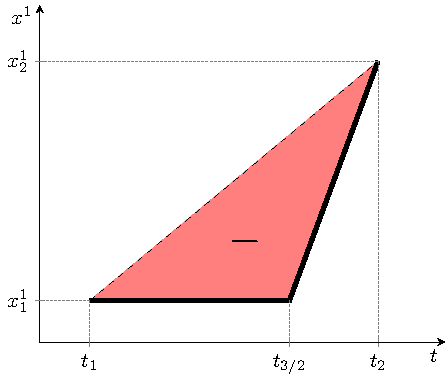
\includegraphics[width=0.45 \columnwidth]{figures/sig_path3.pdf}
    %\vspace{-1.5em}
    \caption{Levy area of forward-fill imputed path.}\label{fig:bentline}
    \vspace{-1em}
\end{figure}

%%%%%%%%%%%%%%%%%%%%%%%%%%%%%%%%%%%%%%%%%%%%%%%%%%%%%%%%%%%%%%%%%%%%%%%%
\subsubsection{Non-causality}
%%%%%%%%%%%%%%%%%%%%%%%%%%%%%%%%%%%%%%%%%%%%%%%%%%%%%%%%%%%%%%%%%%%%%%%%

Once fully observed data has been acquired, either by observation or
data-imputation, then our next operation is always to perform linear
path-imputation.
%
However, linear path-imputation is explicitly non-causal.
%
Given some $(t_i, x_i)$ and $(t_{i+1}, x_{i + 1})$, then the
interpolating function $f$, considered on the interval $(t_i, t_{i
+ 1})$, will already be moving toward $x_{i + 1}$ before that piece of
data has arrived:
%
\begin{equation}
    f(t) = x_{i} \frac{t_{i + 1} - t}{t_{i + 1} - t_i} + x_{i + 1} \frac{t - t_i}{t_{i + 1} - t_i}\text{ for }t \in (t_i, t_{i + 1})
\end{equation}
%
This poses an issue in, for example, the online setting.
%
Non-causality is not always a concern, but we will see in the
next section that the same strategy for overcoming the previous flaw can
overcome this challenge too.
%
% TODO: can we make this into a theorem?
We can summarise this by saying that \emph{when used with the signature transform, any traditional data-imputation scheme will be non-causal}.
% TODO: try and adjust this, it's really the path imputation that's noncausal.

\subsection{Causal signature imputation}
We have spoke so far about the limitations of traditional data-imputation schemes, and at first glance one may be forgiven for thinking that these are issues are unavoidable. 

However, it turns out that we need not be limited just to these traditional imputation schemes. The trick is to consider time not as a \emph{parameterization}, but as a \emph{channel}. Contrast the two possible formulations that were discussed for $\phi$ defined in equation \eqref{eq:phi}.\footnote{To be clear, using time as a channel is already a well-known trick in the signature literature that we do not take credit for inventing! See for example \cite[Definition A.3]{kidger2019deep}. It is however pleasing that something commonly used in the theory of signatures is also what allows us to overcome what we identify as some of their limitations.}

This leads to our novel `meta imputation strategy', which we refer to as \emph{causal signature imputation}. It will turn any traditional causal data-imputation strategy (for example, feed-forward) into a causal path-imputation strategy for signatures; at the same time it will overcome the issue of a fragile dependence.

Suppose we have $\mathbf{x} \in \seriesspace(\dataspace^*)$, and some favourite choice of causal data-imputation strategy $c \colon \seriesspace(\dataspace^*) \to \seriesspace(\dataspace)$.

Next, given
\begin{align*}
    \mathbf{x} = ((t_1, x_1), \ldots, (t_n, x_n)) \in \seriesspace(\dataspace)
\end{align*}
we define the operation $\Phi \colon \seriesspace(\dataspace) \to \seriesspace(\dataspace)$ by
\begin{align}
    \Phi(\mathbf{x}) = (&(t_1, x_1), (t_2, x_1), (t_2, x_2),(t_3, x_2),\nonumber\\
    &\ldots,\nonumber\\
    &(t_i, x_i), (t_{i + 1}, x_i), (t_{i + 1}, x_{i + 1}), (t_{i + 2}, x_{i + 1}),\nonumber\\
    &\ldots,\nonumber\\
    &(t_{n - 1}, x_{n - 1}), (t_n, x_{n - 1}),(t_n, x_n)).\label{eq:causalsig}
\end{align}
That is, first time is updated, and then the corresponding observation in data space is updated. This means that the change in data space occurs instantaneously.

For each $n \in \naturals$ (and given $a < b$), fix any $s_i^{(n)}$ for $i \in \{1, \ldots, n \}$ as in equation \eqref{eq:ss}. (We will see that the exact choice is unimportant in a moment.) Given
\begin{align*}
    \mathbf{x} = ((t_1, x_1), \ldots, (t_n, x_n)) \in \seriesspace(\dataspace),
\end{align*}
let $\psi \colon \seriesspace(\dataspace) \to (\reals \times \dataspace)^{[a, b]}$ be the unique continuous piecewise linear path such that $\psi(s_i^{(n)}) = (t_i, x_i)$. Note that this is just a slight generalisation of the linear path-imputation that has already been performed so far; we are simply no longer asking for additional assumptions of the form $s_i^{(n)} = t_i$.\footnote{As in the $\mathbf{\varphi}_\theta$ of \cite{toth2019gp}, for example.}

Finally, we put this all together, and define the causal signature imputation strategy $\phi_c$ associated with $c$ to be
\begin{equation*}
\phi_c = \psi \circ \Phi \circ c,
\end{equation*}
which will be a map $\seriesspace(\dataspace^*) \to (\reals \times \dataspace)^{[a, b]}$.

Thus $\phi_c$ defines a family of path-imputation schemes, parameterized by a choice of data-imputation scheme.

Why does this work?

First, note that the choice of $s_i^{(n)}$ is unimportant in this definition. By Theorem \ref{theorem:invariancetime}, the signature transform of $\phi_c(\mathbf{x})$ is invariant to this choice.

Second, note that holding time between observations fixed is a valid choice, by the definition for $\seriesspace$ in equation \eqref{eq:seriesspace}. There should hopefully be no moral objection to our definition of $\seriesspace$, as holding time fixed essentially just corresponds to a jump discontinuity; not such a strange thing to have occur. Here, by replacing time as the parameterization, we are then able to recover the continuity of the path.

Third, we claim that $\phi_c$ is immune to both of the flaws we describe in section \ref{section:flaws}. Consider first the flaw of dependence on sampling in unrelated channels.

For simplicity take $c$ to be the forward-fill data-imputation strategy. Consider against the $\mathbf{x}$ defined in expression \eqref{eq:flaw1}. This means that
\begin{equation}\label{eq:causal1}
    \phi_c(\mathbf{x}) = \psi(\;((t_1, x_1^1, x_1^2), (t_2, x_1^1, x_1^2), (t_2, x_2^1, x_1^2))\;).
\end{equation}
% \begin{align*}
%     &\phi_c(\mathbf{x})(s)\\
%     &= \psi(\Phi(c(\mathbf{x})))(s)\\
%     &=\psi(\Phi(\;((t_1, x_1^1, x_1^2), (t_2, x_2^1, C_2))\;))(s)\\
%     &=\psi(\;((t_1, x_1^1, x_1^2), (t_2, x_1^1, x_1^2), (t_2, x_2^1, C_2))\;)(s)\\
%     &= \begin{cases}
%     (t_1 \frac{s_2^{(3)}- s}{s_2^{(3)} - s_1^{(3)}} + t_2 \frac{s - s_1^{(3)}}{s_2^{(3)} - s_1^{(3)}}, x_1^1, x_1^2)\\
%     \hphantom{\hphantom{(t_2, }\,x_1^2 \frac{s_3^{(3)} - s}{s_3^{(3)} - s_2^{(3)}} + C_2 \frac{s - s_2^{(3)}}{s_3^{(3)} - s_2^{(3)}}) }\text{ for }s \in [s_1, s_2]\\
%     (t_2, x_1^1 \frac{s_3^{(3)} - s}{s_3^{(3)} - s_2^{(3)}} + x_2^1 \frac{s - s_2^{(3)}}{s_3^{(3)} - s_2^{(3)}},\\
%     \hphantom{(t_2, }\,x_1^2 \frac{s_3^{(3)} - s}{s_3^{(3)} - s_2^{(3)}} + C_2 \frac{s - s_2^{(3)}}{s_3^{(3)} - s_2^{(3)}}) \text{ for }s \in (s_2, s_3]
%     \end{cases}
% \end{align*}
Contrast adding in the extra observation at $t_{3/2}$ as in equation \eqref{eq:flaw2}. Then
\begin{align}
    &\phi_c(\mathbf{x})(s)\nonumber\\
    &=\psi(\;((t_1, x_1^1, x_1^2), (t_{3/2}, x_1^1, x_1^2), (t_{3/2}, x_1^1, x_{3/2}^2),\nonumber\\ &\hspace{3.1em}(t_2, x_1^1, x_{3/2}^2), (t_2, x_2^1, x_{3/2}^2))\;).\label{eq:causal2}
\end{align}

Evaluating each $\psi$ will then in each case give a path with three channels, corresponding to $t, x^1, x^2$. Then it is clear that the $(t, x^1)$ component of the path in equation \eqref{eq:causal1} is just a reparameterization of the path in equation \eqref{eq:causal2}, a difference which is irrelevant by Theorem \ref{theorem:invariancetime}. (And the $x^2$ component of the second path has been updated to use the new information $x_{3/2}^2$.) Thus the proposed scheme is robust to such issues. For general time series and $c$ taken to be any other causal data-imputation strategy, then much the same analysis can be easily be performed.

Now consider the second potential flaw, of non-causality. The issue previously arose because of the non-causality of the linear path-imputation. We see from equation \eqref{eq:causalsig}, however, such changes only occur in data space while the time channel is frozen; conversely the time channel only updates with the value in the data space frozen. Provided that $c$ is also causal, then causality will, overall, have been preserved. For example, it is possible to use this scheme in an online setting.

There are interesting comparisons to be made between causal signature imputation and certain operations in the signature literature. First is the \emph{lead-lag} transform \cite{primer2016}. With the lead-lag transform, the entire path is \emph{duplicated}, and then each side is alternately updated. Conversely, in causal signature imputation, the path is instead \emph{split} between $t$ and $(x^1, \ldots, x^n)$, and then each side is alternately updated.

Second is the comparison to the linear and rectilinear embedding strategies, see for example \cite{fermanian2019embedding}. It is possible to interpret $\psi \circ \Phi$ as a hybrid between the linear and rectilinear embeddings: it is rectilinear with respect to an ordering of $t$ and $(x^1, \ldots, x^n)$, and linear on $(x^1, \ldots, x^n)$.

\subsection{Extending Gaussian process adapters with posterior moments}\label{section:ourgpadapter}
TODO: % emphasize that the idea behind the PoM is that the model has access to uncertainty information during the prediction step. We argue that the previous formulation is not really uncertainty-aware in this sense, and we propose an approach to fix this. Notably, PoM comes at the cost of losing uncertainty \emph{about} the models predictions. 

Non-causality is not necessarily a worrying flaw, especially when not operating in an online setting. As such, we go on to consider another promising, but non-causal, path-imputation method, by adapting the Gaussian process adapter described in section \ref{section:gpadapter}.

One major drawback with the formulations of \cite{li2016scalable} and \cite{futoma2017mgp}, as described in equation \eqref{eq:gp-mc}, is that approximating the expectation outside of the loss function with Monte Carlo sampling is expensive.

During prediction, they propose to overcome this issue by sacrificing the uncertainty in the loss function and to simply pass the posterior mean, as in \eqref{eq:gp-mean}.\footnote{Equations \eqref{eq:gp-mc} and \eqref{eq:gp-mean} are of course not in general equal, so really the same procedure should be used for both training and test -- despite the description given in \cite[Section 3.1]{li2016scalable}.}

To address both points, we propose to instead also pass the posterior covariance of the Gaussian process to the classifier $F$. This saves the cost of Monte Carlo sampling whilst explicitly providing the classifier with $F$ with uncertainty information.

However, full covariance matrices may become very large, with much of it not obviously helpful to the subsequent classifier. We instead simplify matters by taking the posterior variance at every point, and concatenate it with the posterior mean at every point, to produce a path whose evolution describes the uncertainty at every point:
\begin{align*}
    \tau &\colon [a, b] \times \seriesspace(\dataspace^*) \times \mathcal{H} \to \dataspace \times \dataspace\\
    \tau &\colon t, \mathbf{x}, \eta \mapsto (\mu(t, \mathbf{x}, \eta), \Sigma(t, t, \mathbf{x}, \eta)).
\end{align*}

This corresponds to solving
\begin{equation}\label{eq:gp-moments}
\argmin_{\mathbf{w} \in \mathcal{W},\bm{\eta} \in \mathcal{H}} \sum_{k=1}^N \ell(F(\tau(\,\cdot\,,\mathbf{x}_k, \eta), \mathbf{w}), y_k),
\end{equation}
where instead now
\begin{equation*}
    F \colon (\dataspace \times \dataspace)^{[a, b]} \times \mathcal{W} \to \lspace.
\end{equation*}

Training this model is no harder than the formulation of \cite{li2016scalable}. Abusing notation by conflating the Gaussian process sample $\mathbf{z}$ with its finite dimensional distribution that is of interest, simply decompose $\mathbf{z} = \mu + R \xi$, with $\xi$ a standard multivariate normal and $R$ such that $\Sigma = RR^T$. The derivatives of equation \eqref{eq:gp-moments} are now no harder to describe than they were before.

In our context of interest, when $F$ is a signature model, then it is now straightforward to compute the signature of the Gaussian process, simply by sampling many points to construct a piecewise linear approximation to the process. Technically speaking, the choice of kernel has nontrivial mathematical implications for this procedure: for example if a Mat{\'e}rn 1/2 kernel is chosen, then the resulting path is not of bounded variation and the definition of the signature transform given in equation \eqref{eq:signature} does not hold, and rough path theory \cite{lyons1998differential} must instead be invoked to define the signature transform.

This formulation, whilst lacking causality, is nonetheless robust to the issue of fragility with respect to observations in unrelated channels. The Gaussian process adapter operates globally on all observed data, and observations in unrelated channels are allowed to be uncorrelated. This framework is also naturally more powerful at modelling than the explicit parameter-free schemes discussed thus far.

\section{Experiments}
% The flaws we have identified have been theoretically identified, and so we have been able to correct them theoretically as well. Nonetheless we have also performed experiments, testing different imputation schemes across several different signature-based models.
For our empirical analysis, let us first introduce our experimental setup by specifying the investigated datasets, models, imputation schemes as well as prediction tasks at hand. Subsequently, we present and discuss our quantitative results.
\subsection{Datasets}
We make use of four real-world time series datasets: Physionet2012 challenge \cite{goldberger2000physiobank},
    PenDigits \cite{Dua2019}, LSST \cite{allam2018photometric}, and CharacterTrajectories \cite{Dua2019}.

\subsection{Models}
We study the following set of models:
\begin{enumerate}
    \item Sig, a simple signature model which involves a linear augmentation, the signature transform (signature block) and a final module of dense layers.
    \item RNNSig, which extends the signature transform to a window-based stream of signatures, and where the final neural module is a GRU sliding over the stream of signatures.
    %\item DeepSig, where two signature blocks are stacked.
    \item RNN, a straight-forward RNN model using gated recurrent units (GRU) as RNN cells.
\end{enumerate}
For more details with respect to architectures and implemenation, please refer to the supplementary Sectoin XXXX.
First, we examined the PhysioNet 2012 Mortality Prediction Dataset.

We performed several experiments, testing different imputation schemes across several different signature models.
To calculate the signature transform, we used the Signatory package of \cite{signatory}.

\begin{figure*}[tbp]
  \subcaptionbox{CharacterTrajectories-R}{%
    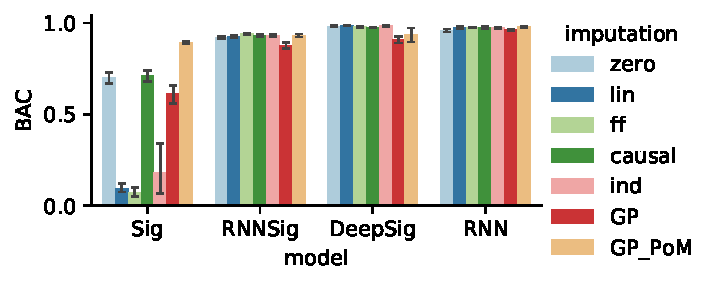
\includegraphics[width=0.48\linewidth]{plots/barplot_main_CharacterTrajectories-MissingAtRandomSubsampler.pdf}\quad%
    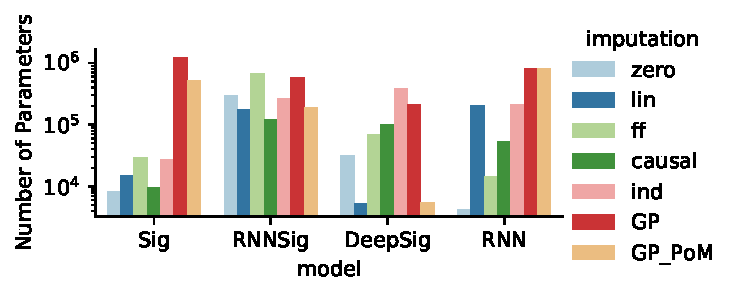
\includegraphics[width=0.48\linewidth]{plots/barplot_main_params_CharacterTrajectories-MissingAtRandomSubsampler.pdf}%
  }\\%
  \subcaptionbox{CharacterTrajectories-L}{%
    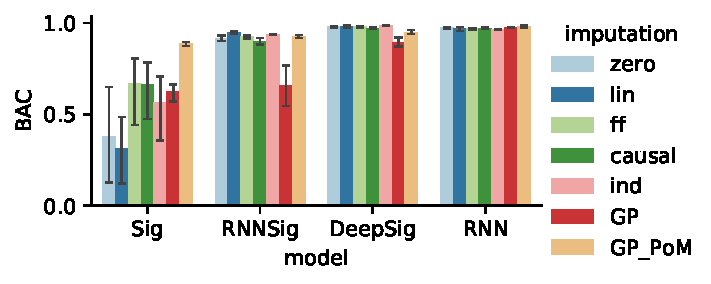
\includegraphics[width=0.48\linewidth]{plots/barplot_main_CharacterTrajectories-LabelBasedSubsampler.pdf}\quad%
    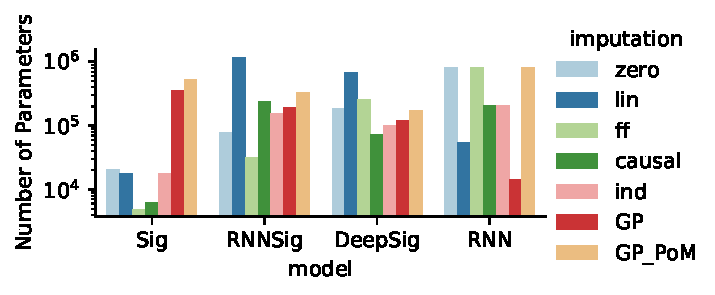
\includegraphics[width=0.48\linewidth]{plots/barplot_main_params_CharacterTrajectories-LabelBasedSubsampler.pdf}%
  }\\%
  \subcaptionbox{LSST-R}{%
    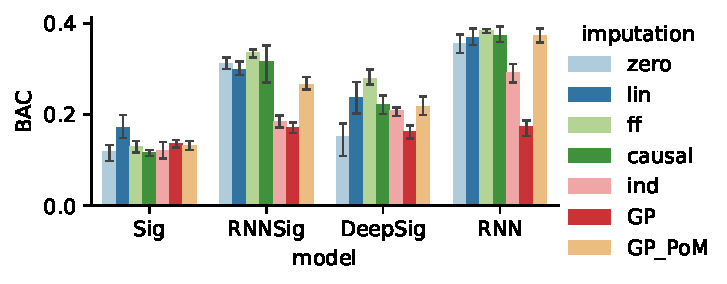
\includegraphics[width=0.48\linewidth]{plots/barplot_main_LSST-MissingAtRandomSubsampler.pdf}\quad%
    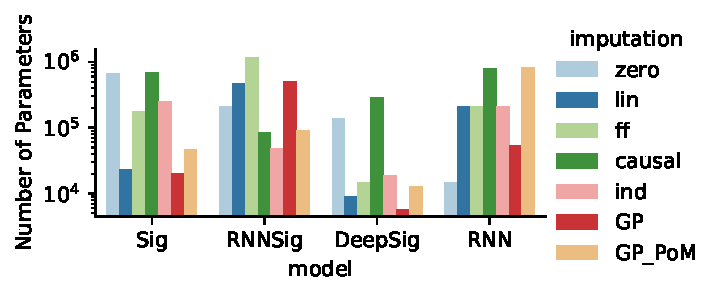
\includegraphics[width=0.48\linewidth]{plots/barplot_main_params_LSST-MissingAtRandomSubsampler.pdf}%
  }\\%
  \subcaptionbox{LSST-L}{%
    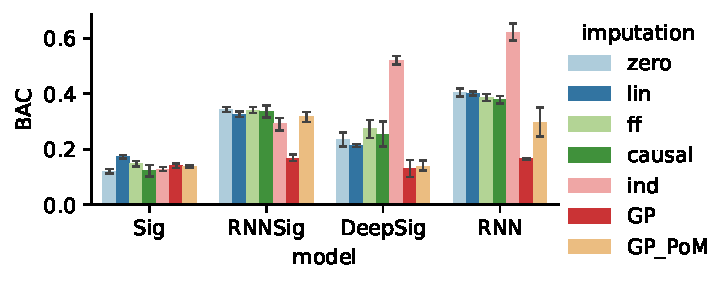
\includegraphics[width=0.48\linewidth]{plots/barplot_main_LSST-LabelBasedSubsampler.pdf}\quad%
    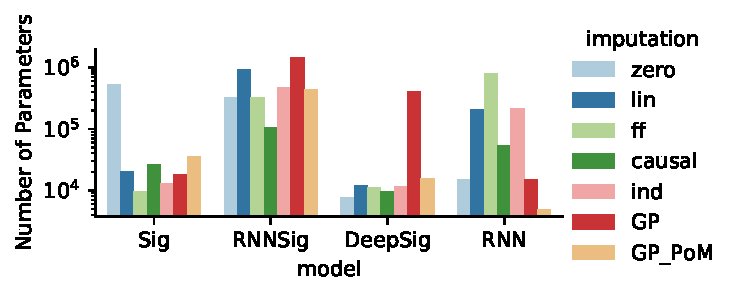
\includegraphics[width=0.48\linewidth]{plots/barplot_main_params_LSST-LabelBasedSubsampler.pdf}
  }\\%
   \subcaptionbox{PenDigits-R}{%
     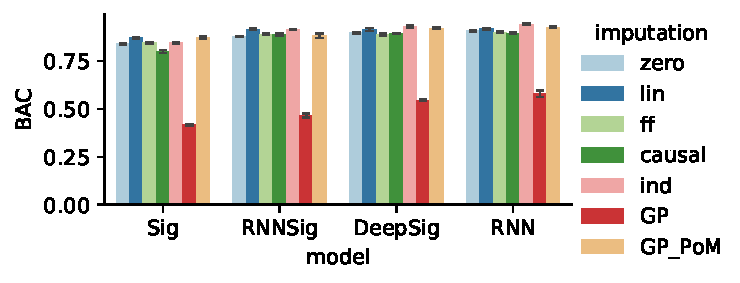
\includegraphics[width=0.48\linewidth]{plots/barplot_main_PenDigits-MissingAtRandomSubsampler.pdf}\quad%
     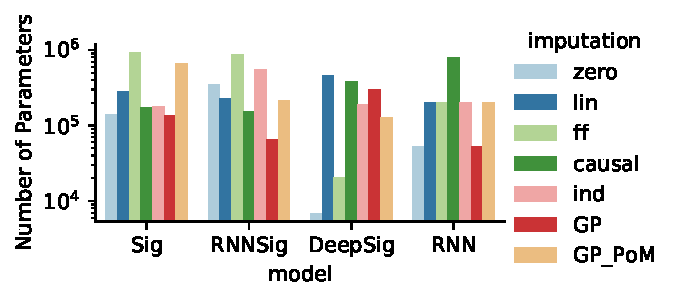
\includegraphics[width=0.48\linewidth]{plots/barplot_main_params_PenDigits-MissingAtRandomSubsampler.pdf}
   }\\%
  \subcaptionbox{PenDigits-L}{%
    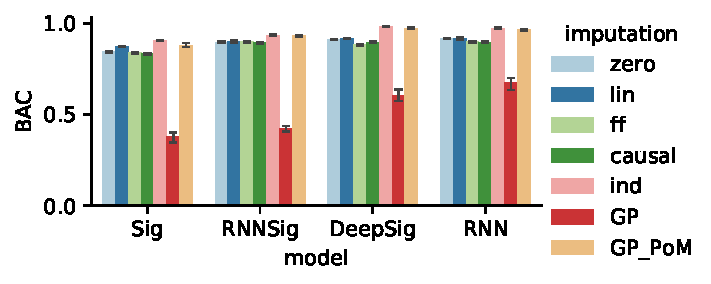
\includegraphics[width=0.48\linewidth]{plots/barplot_main_PenDigits-LabelBasedSubsampler.pdf}\quad%
    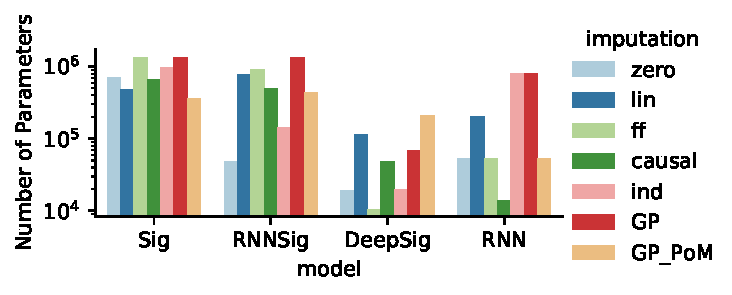
\includegraphics[width=0.48\linewidth]{plots/barplot_main_params_PenDigits-LabelBasedSubsampler.pdf}
  }\\ %
  \subcaptionbox{Physionet2012}{%
    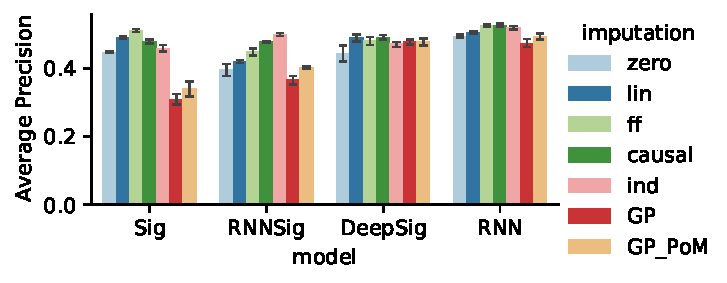
\includegraphics[width=0.48\linewidth]{plots/barplot_main_Physionet2012-.pdf}\quad%
    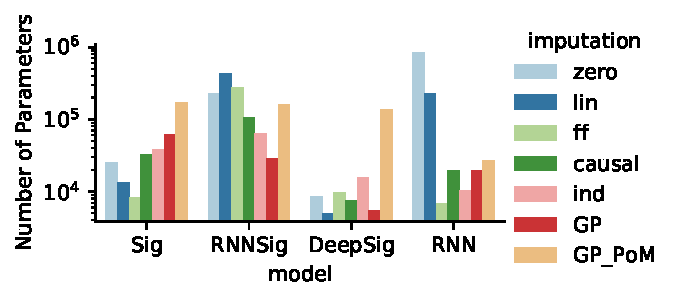
\includegraphics[width=0.48\linewidth]{plots/barplot_main_params_Physionet2012-.pdf}
  }
  \caption{%
    Experimental results.
  }
  \label{fig: barplots}
\end{figure*}

{\tiny
\begin{table}[h]
    \caption{\textbf{Physionet 2012}. The below methods are named as $<$imputation method$>-<$prediction model$>$. GP indicates an end-to-end trained Gaussian Process adapter, whereas PoM indicates our proposed extension, "posterior moments". The remaining imputation schemes have been applied as a preprocessing step, whereas the abbreviations "causal, ff, ind, lin, and zero" refer to: "causal, forward-filling, indicator, linear, and zero". Highlighting of the 3 best methods in decreasing order: bold as well as underlined, bold, and underlined.}
    \begin{tabular}{lll}
\toprule
metric &                                 AUROC &                     Average Precision \\
model            &                                       &                                       \\
\midrule
GP-DeepSig       &                           $ 0.83057 $ &                           $ 0.48053 $ \\
GP-DeepSig (PoM) &                            $ 0.8202 $ &                           $ 0.49333 $ \\
GP-RNN           &                           $ 0.82501 $ &                           $ 0.48862 $ \\
GP-RNN (PoM)     &                            $ 0.8411 $ &                           $ 0.50316 $ \\
GP-RNNSig        &                           $ 0.75912 $ &                           $ 0.36152 $ \\
GP-RNNSig (PoM)  &                           $ 0.77133 $ &                            $ 0.4031 $ \\
GP-Sig           &                           $ 0.73406 $ &                           $ 0.35228 $ \\
GP-Sig (PoM)     &                           $ 0.76132 $ &                           $ 0.34929 $ \\
causal-DeepSig   &                           $ 0.83786 $ &                           $ 0.49095 $ \\
causal-RNN       &               $  \mathbf{ 0.84687 } $ &               $  \mathbf{ 0.51729 } $ \\
causal-RNNSig    &                           $ 0.81896 $ &                           $ 0.46484 $ \\
causal-Sig       &                           $ 0.83908 $ &                           $ 0.48984 $ \\
ff-DeepSig       &                           $ 0.82189 $ &                           $ 0.48037 $ \\
ff-RNN           &            $  \underline{ 0.84655 } $ &  $  \mathbf{ \underline{ 0.52581 }} $ \\
ff-RNNSig        &                           $ 0.80963 $ &                           $ 0.43971 $ \\
ff-Sig           &                           $ 0.84356 $ &                            $ 0.5036 $ \\
ind-DeepSig      &                           $ 0.82432 $ &                           $ 0.48006 $ \\
ind-RNN          &  $  \mathbf{ \underline{ 0.84961 }} $ &            $  \underline{ 0.51611 } $ \\
ind-RNNSig       &                           $ 0.83766 $ &                           $ 0.50512 $ \\
ind-Sig          &                           $ 0.80753 $ &                           $ 0.46094 $ \\
lin-DeepSig      &                            $ 0.8338 $ &                           $ 0.49465 $ \\
lin-RNN          &                           $ 0.84303 $ &                           $ 0.51061 $ \\
lin-RNNSig       &                            $ 0.7769 $ &                           $ 0.42146 $ \\
lin-Sig          &                           $ 0.83442 $ &                           $ 0.49693 $ \\
zero-DeepSig     &                           $ 0.82405 $ &                           $ 0.47245 $ \\
zero-RNN         &                           $ 0.84041 $ &                           $ 0.49561 $ \\
zero-RNNSig      &                           $ 0.78151 $ &                           $ 0.41783 $ \\
zero-Sig         &                           $ 0.80593 $ &                           $ 0.44305 $ \\
\bottomrule
\end{tabular}
 %TODO: I need to update the result tables with repetitions including std estimates (curerntly hyperparameter search results - not repetitions.
\end{table}
}


\section{Recommendations}
We finish with some recommendations for the practitioner, based on our findings.

Whether causality is a concern or not, then causal signature imputation is simple to implement and effective at correcting the identified issues. If one takes the point of view that the signature transform is defined on data (rather than paths), then all that is necessary is to pick one's favourite imputation scheme, apply it as usual, and then apply the $\Phi$ of equation \eqref{eq:phi} to the imputed data, before using it. In more complicated models such as those proposed by \cite{kidger2019deep}, then a perfectly valid `zero thought' approach is to precompose $\Phi$ of equation \eqref{eq:phi} to every usage of the signature transform.

If causality is not a concern, then we recommend the variation of a Gaussian process adapter proposed in section \ref{section:ourgpadapter}. The implementation of this is much less straightforward, however. It remains a reasonable compromise to use linear data-imputation, which is unique in avoiding the flaw of dependence on unrelated channels, whilst accepting that there may be slight inconsistencies at either end of a partially observed time series.

We do not recommend applying any standard imputation scheme unless it has been modified by causal signature imputation.

\section{Conclusion}
When using the signature transform in machine learning, we have identified a novel issue in the greater-than-usual importance of the choice of imputation strategy.

We have identified two key flaws that can arise when mishandling this issue, and show that they are necessarily exhibited by all conventional imputation strategies not specifically adapted for use with the signature transform.

We have then proposed two practical, novel, solutions to overcome them,
namely causal signature imputation and a Gaussian process adapter, the
latter of which is of independent interest in other scenarios due to the
way it incorporates uncertainty information about the \emph{predictions}
themselves.

As a result, we are able to summarise with `recommendations for the practitioner' on the appropriateness of different techniques.

\section*{Broader Impact}
TODO

\begin{ack}
TODO
\end{ack}

\bibliography{ref}
\bibliographystyle{apalike} %ieeetr
\newpage
\appendix

\section{Appendix}\label{sec:Appendix}

\section{Fragile dependence on sampling in unrelated channels: example}%
\label{sec:Fragile dependence} 

Suppose that we have observed the (very short) time series
\begin{equation}\label{eq:flaw1}
    \mathbf{x} = ((t_1, x_1^1, x_1^2), (t_2, x_2^1, *)) \in \seriesspace(\reals^2).
\end{equation}
Perhaps we now apply, say, forward fill data-imputation, to produce
\begin{equation*}
    ((t_1, x_1^1, x_1^2), (t_2, x_2^1, x_1^2)).
\end{equation*}
Finally we linearly path-impute to create the linear path
\begin{align*}
    f &\colon [t_1, t_2] \to \reals \times \reals^2\\
    f &\colon t \mapsto (t, x_1^1\frac{t_2 - t}{t_2 - t_1} + x_2^1\frac{t - t_1}{t_2 - t_1}, x_1^2),
\end{align*}
to which we may then apply the signature transform. In particular we will have computed the Levy area with respect to $t$ and $x^1$. As this is just a straight line, the Levy area is zero.

Now suppose we include an additional observation at some time $t_{3/2} \in (t_1, t_2)$, so that our data is instead
\begin{equation}\label{eq:flaw2}
    \mathbf{x} = ((t_1, x_1^1, x_1^2), (t_{3/2}, *, x_{3/2}^2), (t_2, x_2^1, *)).
\end{equation}
Then the same procedure as before will produce the data
\begin{equation*}
    \mathbf{x} = ((t_1, x_1^1, x_1^2), (t_{3/2}, x_1^1, x_{3/2}^2), (t_2, x_2^1, x_{3/2}^2)),
\end{equation*}
with corresponding function $f$. The $(t, x^1)$ components of $f$ and its $(t, x^1)$-Levy area are shown in Figure \ref{fig:bentline}. As a result of an unrelated observation in the $x^2$ channel, the $(t, x^1)$-Levy area has been changed. The closer $t_{3/2}$ is to $t_2$, the greater the disparity.

This simple example underscores the danger of `just forward-fill data-imputing'. Doing so has introduced an undesired dependency on the simple \emph{presence} of an observation in other channels, with the change in our imputed path being determined by the \emph{time} at which this other observation occurred.

Indeed, any imputation scheme that predicts something other than the unique value lying on the dashed line in Figure \ref{fig:bentline}, will fail. This means that this example holds for essentially every data-imputation scheme -- the only scheme that survives this flaw is the linear data-imputation scheme. This is the unique imputation scheme which coincides with the linear path-imputation that \emph{must} be our concluding step.

% Extending our previous example, linear data-imputation would produce
% \begin{align*}
%     \mathbf{x} = (&(t_1, x_1^1, x_1^2),\\
%     &(t_{3/2}, x_1^1 \frac{t_2 - t_{3/2}}{t_2 - t_1} + x_2^1 \frac{t_{3/2} - t_1}{t_2 - t_1}, x_{3/2}^2),\\
%     &(t_2, x_2^1, *)).
% \end{align*}
% Note that there is still an unimputed piece of data in the $x_2^2$ slot; we will return to this in a moment. Concerning the $x_{3/2}^1$ slot, we see that the value imputed is precisely the same as that given by a subsequent linear path-imputation, and it is in this way that the linear scheme does not fall afoul of this flaw.

However, when there is missing data at the start or the end of a partially observed times series, then there is no `next observation' which linear imputation can use. So in general, we cannot uniformly apply the linear data-imputation scheme, and must choose another scheme.

\subsection{Further Experiments}\label{supp:Experiments}
Describe here the further datasets, the subsampling types etc.

\begin{table*}
    \begin{center}
	\caption{PenDigits}
	\begin{tabular}{lllll}
\toprule
       & metric &                               w-AUROC &                                   BAC &                              Accuracy \\
subsampling & model &                                       &                                       &                                       \\
\midrule
Label-based & GP-DeepSig &                           $ 0.88296 $ &                           $ 0.49497 $ &                           $ 0.49434 $ \\
       & GP-DeepSig (PoM) &            $  \underline{ 0.99933 } $ &            $  \underline{ 0.97306 } $ &            $  \underline{ 0.97313 } $ \\
       & GP-RNN &                           $ 0.90424 $ &                           $ 0.54095 $ &                           $ 0.53979 $ \\
       & GP-RNN (PoM) &                           $ 0.99899 $ &                           $ 0.96359 $ &                           $ 0.96341 $ \\
       & GP-RNNSig &                           $ 0.85031 $ &                           $ 0.43521 $ &                           $ 0.43436 $ \\
       & GP-RNNSig (PoM) &                           $ 0.99707 $ &                           $ 0.93331 $ &                           $ 0.93282 $ \\
       & GP-Sig &                           $ 0.81601 $ &                           $ 0.39828 $ &                           $ 0.39863 $ \\
       & GP-Sig (PoM) &                           $ 0.99148 $ &                           $ 0.88778 $ &                           $ 0.88708 $ \\
       & causal-DeepSig &                           $ 0.99308 $ &                           $ 0.89909 $ &                           $ 0.89794 $ \\
       & causal-RNN &                           $ 0.99255 $ &                           $ 0.89727 $ &                           $ 0.89651 $ \\
       & causal-RNNSig &                           $ 0.99308 $ &                           $ 0.88905 $ &                           $ 0.88822 $ \\
       & causal-Sig &                           $ 0.98389 $ &                           $ 0.83694 $ &                           $ 0.83591 $ \\
       & ff-DeepSig &                           $ 0.98934 $ &                           $ 0.89039 $ &                           $ 0.88908 $ \\
       & ff-RNN &                            $ 0.9933 $ &                           $ 0.90463 $ &                           $ 0.90395 $ \\
       & ff-RNNSig &                           $ 0.99351 $ &                           $ 0.89911 $ &                            $ 0.8988 $ \\
       & ff-Sig &                           $ 0.98248 $ &                           $ 0.83489 $ &                           $ 0.83362 $ \\
       & ind-DeepSig &               $  \mathbf{ 0.99941 } $ &  $  \mathbf{ \underline{ 0.97713 }} $ &  $  \mathbf{ \underline{ 0.97684 }} $ \\
       & ind-RNN &  $  \mathbf{ \underline{ 0.99951 }} $ &               $  \mathbf{ 0.97369 } $ &                $  \mathbf{ 0.9737 } $ \\
       & ind-RNNSig &                           $ 0.99732 $ &                           $ 0.92969 $ &                            $ 0.9291 $ \\
       & ind-Sig &                           $ 0.99325 $ &                           $ 0.89804 $ &                           $ 0.89737 $ \\
       & lin-DeepSig &                           $ 0.99567 $ &                           $ 0.92518 $ &                           $ 0.92424 $ \\
       & lin-RNN &                           $ 0.99539 $ &                           $ 0.92628 $ &                           $ 0.92567 $ \\
       & lin-RNNSig &                           $ 0.99495 $ &                           $ 0.90451 $ &                           $ 0.90366 $ \\
       & lin-Sig &                           $ 0.99041 $ &                           $ 0.87628 $ &                           $ 0.87479 $ \\
       & zero-DeepSig &                           $ 0.99274 $ &                           $ 0.90518 $ &                           $ 0.90395 $ \\
       & zero-RNN &                           $ 0.99586 $ &                           $ 0.92182 $ &                            $ 0.9211 $ \\
       & zero-RNNSig &                           $ 0.99326 $ &                            $ 0.8939 $ &                           $ 0.89308 $ \\
       & zero-Sig &                           $ 0.98303 $ &                           $ 0.83421 $ &                           $ 0.83305 $ \\
Random & GP-DeepSig &                           $ 0.90964 $ &                           $ 0.55605 $ &                           $ 0.55563 $ \\
       & GP-DeepSig (PoM) &                           $ 0.99527 $ &                           $ 0.92081 $ &                           $ 0.92024 $ \\
       & GP-RNN &                           $ 0.90783 $ &                           $ 0.54607 $ &                           $ 0.54594 $ \\
       & GP-RNN (PoM) &                           $ 0.99578 $ &            $  \underline{ 0.92919 } $ &            $  \underline{ 0.92853 } $ \\
       & GP-RNNSig &                           $ 0.86954 $ &                           $ 0.47817 $ &                           $ 0.47802 $ \\
       & GP-RNNSig (PoM) &                           $ 0.99336 $ &                            $ 0.9066 $ &                           $ 0.90595 $ \\
       & GP-Sig &                           $ 0.84778 $ &                           $ 0.44101 $ &                             $ 0.442 $ \\
       & GP-Sig (PoM) &                           $ 0.98924 $ &                           $ 0.87698 $ &                           $ 0.87679 $ \\
       & causal-DeepSig &                           $ 0.99262 $ &                           $ 0.89371 $ &                           $ 0.89308 $ \\
       & causal-RNN &                            $ 0.9925 $ &                           $ 0.89175 $ &                           $ 0.89165 $ \\
       & causal-RNNSig &                           $ 0.99115 $ &                           $ 0.88842 $ &                           $ 0.88794 $ \\
       & causal-Sig &                           $ 0.98249 $ &                           $ 0.82081 $ &                            $ 0.8199 $ \\
       & ff-DeepSig &                           $ 0.99055 $ &                           $ 0.88501 $ &                           $ 0.88451 $ \\
       & ff-RNN &                           $ 0.99419 $ &                           $ 0.90398 $ &                           $ 0.90337 $ \\
       & ff-RNNSig &                            $ 0.9922 $ &                           $ 0.88938 $ &                           $ 0.88908 $ \\
       & ff-Sig &                           $ 0.98571 $ &                           $ 0.84269 $ &                           $ 0.84191 $ \\
       & ind-DeepSig &                $  \mathbf{ 0.9972 } $ &               $  \mathbf{ 0.93715 } $ &               $  \mathbf{ 0.93654 } $ \\
       & ind-RNN &  $  \mathbf{ \underline{ 0.99771 }} $ &  $  \mathbf{ \underline{ 0.94814 }} $ &  $  \mathbf{ \underline{ 0.94768 }} $ \\
       & ind-RNNSig &                           $ 0.99562 $ &                           $ 0.91775 $ &                            $ 0.9171 $ \\
       & ind-Sig &                           $ 0.98783 $ &                           $ 0.84821 $ &                           $ 0.84763 $ \\
       & lin-DeepSig &                           $ 0.99438 $ &                           $ 0.91783 $ &                           $ 0.91767 $ \\
       & lin-RNN &                           $ 0.99463 $ &                           $ 0.91445 $ &                           $ 0.91395 $ \\
       & lin-RNNSig &            $  \underline{ 0.99621 } $ &                           $ 0.92118 $ &                           $ 0.92081 $ \\
       & lin-Sig &                           $ 0.99149 $ &                            $ 0.8843 $ &                           $ 0.88393 $ \\
       & zero-DeepSig &                             $ 0.994 $ &                           $ 0.90535 $ &                           $ 0.90452 $ \\
       & zero-RNN &                            $ 0.9955 $ &                           $ 0.91814 $ &                           $ 0.91795 $ \\
       & zero-RNNSig &                           $ 0.99113 $ &                           $ 0.88433 $ &                           $ 0.88422 $ \\
       & zero-Sig &                           $ 0.98705 $ &                           $ 0.83734 $ &                           $ 0.83648 $ \\
\bottomrule
\end{tabular}

	\end{center}
\end{table*}

\newpage

\begin{table*}
    \begin{center}
	\caption{LSST}
	\begin{tabular}{lllll}
\toprule
       & metric &                               w-AUROC &                                   BAC &                             Accuracy \\
subsampling & model &                                       &                                       &                                      \\
\midrule
Label-based & GP-DeepSig &                           $ 0.63585 $ &                           $ 0.18197 $ &                          $ 0.21999 $ \\
       & GP-DeepSig (PoM) &                           $ 0.74772 $ &                           $ 0.15754 $ &                           $ 0.1326 $ \\
       & GP-RNN &                            $ 0.6751 $ &                           $ 0.17692 $ &                          $ 0.34071 $ \\
       & GP-RNN (PoM) &            $  \underline{ 0.90377 } $ &                           $ 0.39123 $ &                          $ 0.46472 $ \\
       & GP-RNNSig &                           $ 0.60471 $ &                           $ 0.15081 $ &                          $ 0.33479 $ \\
       & GP-RNNSig (PoM) &                           $ 0.82478 $ &                           $ 0.28931 $ &                          $ 0.30089 $ \\
       & GP-Sig &                           $ 0.57096 $ &                            $ 0.1343 $ &                          $ 0.23946 $ \\
       & GP-Sig (PoM) &                           $ 0.59807 $ &                           $ 0.16114 $ &                         $ 0.095702 $ \\
       & causal-DeepSig &                           $ 0.80577 $ &                            $ 0.3125 $ &                          $ 0.48459 $ \\
       & causal-RNN &                           $ 0.84624 $ &                           $ 0.33731 $ &                          $ 0.53082 $ \\
       & causal-RNNSig &                           $ 0.82314 $ &                           $ 0.32955 $ &                          $ 0.51338 $ \\
       & causal-Sig &                           $ 0.59027 $ &                           $ 0.13125 $ &                          $ 0.33536 $ \\
       & ff-DeepSig &                           $ 0.75571 $ &                            $ 0.2625 $ &                          $ 0.34712 $ \\
       & ff-RNN &                           $ 0.84691 $ &                           $ 0.38555 $ &                          $ 0.53569 $ \\
       & ff-RNNSig &                           $ 0.82531 $ &                           $ 0.35215 $ &                          $ 0.48418 $ \\
       & ff-Sig &                           $ 0.63727 $ &                           $ 0.14316 $ &                           $ 0.3459 $ \\
       & ind-DeepSig &               $  \mathbf{ 0.95327 } $ &               $  \mathbf{ 0.51621 } $ &              $  \mathbf{ 0.80535 } $ \\
       & ind-RNN &  $  \mathbf{ \underline{ 0.98128 }} $ &  $  \mathbf{ \underline{ 0.59382 }} $ &  $  \mathbf{ \underline{ 0.8232 }} $ \\
       & ind-RNNSig &                           $ 0.81609 $ &                           $ 0.31671 $ &                          $ 0.41403 $ \\
       & ind-Sig &                           $ 0.57659 $ &                           $ 0.12875 $ &                          $ 0.33901 $ \\
       & lin-DeepSig &                           $ 0.76319 $ &                           $ 0.27597 $ &                          $ 0.46067 $ \\
       & lin-RNN &                           $ 0.84534 $ &                           $ 0.37092 $ &                          $ 0.53893 $ \\
       & lin-RNNSig &                           $ 0.83496 $ &                           $ 0.34416 $ &                          $ 0.52555 $ \\
       & lin-Sig &                           $ 0.66955 $ &                           $ 0.17077 $ &                          $ 0.36253 $ \\
       & zero-DeepSig &                           $ 0.74004 $ &                           $ 0.23683 $ &                          $ 0.33171 $ \\
       & zero-RNN &                           $ 0.89525 $ &            $  \underline{ 0.40892 } $ &           $  \underline{ 0.54663 } $ \\
       & zero-RNNSig &                           $ 0.78403 $ &                           $ 0.31934 $ &                          $ 0.46513 $ \\
       & zero-Sig &                            $ 0.5493 $ &                           $ 0.15275 $ &                          $ 0.30616 $ \\
Random & GP-DeepSig &                           $ 0.62195 $ &                           $ 0.15651 $ &                          $ 0.34643 $ \\
       & GP-DeepSig (PoM) &                           $ 0.74952 $ &                           $ 0.29438 $ &                          $ 0.36537 $ \\
       & GP-RNN &                           $ 0.64693 $ &                            $ 0.1847 $ &                          $ 0.35223 $ \\
       & GP-RNN (PoM) &                           $ 0.82287 $ &                           $ 0.36185 $ &                            $ 0.515 $ \\
       & GP-RNNSig &                           $ 0.60061 $ &                           $ 0.18232 $ &                          $ 0.33755 $ \\
       & GP-RNNSig (PoM) &                           $ 0.77488 $ &                           $ 0.27175 $ &                          $ 0.43674 $ \\
       & GP-Sig &                           $ 0.58776 $ &                            $ 0.1462 $ &                          $ 0.33228 $ \\
       & GP-Sig (PoM) &                            $ 0.5963 $ &                           $ 0.12667 $ &                          $ 0.35036 $ \\
       & causal-DeepSig &                           $ 0.77341 $ &                           $ 0.26873 $ &                          $ 0.32157 $ \\
       & causal-RNN &  $  \mathbf{ \underline{ 0.84593 }} $ &            $  \underline{ 0.37103 } $ &  $  \mathbf{ \underline{ 0.5661 }} $ \\
       & causal-RNNSig &                           $ 0.80265 $ &  $  \mathbf{ \underline{ 0.38461 }} $ &                          $ 0.50527 $ \\
       & causal-Sig &                           $ 0.55507 $ &                           $ 0.16425 $ &                          $ 0.33049 $ \\
       & ff-DeepSig &                           $ 0.75865 $ &                           $ 0.26642 $ &                          $ 0.26237 $ \\
       & ff-RNN &                 $  \mathbf{ 0.841 } $ &               $  \mathbf{ 0.37914 } $ &              $  \mathbf{ 0.55191 } $ \\
       & ff-RNNSig &                           $ 0.82349 $ &                           $ 0.35866 $ &                          $ 0.49635 $ \\
       & ff-Sig &                           $ 0.56967 $ &                           $ 0.12029 $ &                          $ 0.33901 $ \\
       & ind-DeepSig &                           $ 0.64712 $ &                           $ 0.17605 $ &                          $ 0.34347 $ \\
       & ind-RNN &                           $ 0.79579 $ &                           $ 0.31312 $ &                          $ 0.46634 $ \\
       & ind-RNNSig &                           $ 0.64653 $ &                           $ 0.18762 $ &                          $ 0.30616 $ \\
       & ind-Sig &                           $ 0.52971 $ &                           $ 0.11215 $ &                          $ 0.32036 $ \\
       & lin-DeepSig &                           $ 0.78331 $ &                           $ 0.25471 $ &                          $ 0.43512 $ \\
       & lin-RNN &            $  \underline{ 0.83925 } $ &                           $ 0.36831 $ &           $  \underline{ 0.54745 } $ \\
       & lin-RNNSig &                           $ 0.82926 $ &                           $ 0.31372 $ &                          $ 0.51135 $ \\
       & lin-Sig &                           $ 0.66071 $ &                           $ 0.18364 $ &                          $ 0.37713 $ \\
       & zero-DeepSig &                           $ 0.73129 $ &                           $ 0.20532 $ &                            $ 0.412 $ \\
       & zero-RNN &                            $ 0.8197 $ &                           $ 0.33041 $ &                           $ 0.5219 $ \\
       & zero-RNNSig &                           $ 0.78279 $ &                           $ 0.32638 $ &                          $ 0.45904 $ \\
       & zero-Sig &                           $ 0.54915 $ &                           $ 0.15811 $ &                         $ 0.076237 $ \\
\bottomrule
\end{tabular}

	\end{center}
\end{table*}

\newpage

\begin{table*}
    \begin{center}
	\caption{Character Trajectories }
	\begin{tabular}{lllll}
\toprule
       & metric &                               w-AUROC &                                   BAC &                              Accuracy \\
subsampling & model &                                       &                                       &                                       \\
\midrule
Label-based & GP-DeepSig &                           $ 0.99852 $ &                           $ 0.93516 $ &                           $ 0.93273 $ \\
       & GP-DeepSig (PoM) &                           $ 0.99956 $ &                           $ 0.97529 $ &                           $ 0.97772 $ \\
       & GP-RNN &                           $ 0.99937 $ &                           $ 0.96977 $ &                           $ 0.97208 $ \\
       & GP-RNN (PoM) &               $  \mathbf{ 0.99993 } $ &            $  \underline{ 0.98933 } $ &            $  \underline{ 0.98955 } $ \\
       & GP-RNNSig &                           $ 0.98492 $ &                           $ 0.76234 $ &                           $ 0.77019 $ \\
       & GP-RNNSig (PoM) &                           $ 0.99706 $ &                           $ 0.94428 $ &                           $ 0.94708 $ \\
       & GP-Sig &                           $ 0.97624 $ &                           $ 0.73415 $ &                           $ 0.74088 $ \\
       & GP-Sig (PoM) &                           $ 0.99626 $ &                           $ 0.90547 $ &                           $ 0.90877 $ \\
       & causal-DeepSig &                            $ 0.9991 $ &                             $ 0.975 $ &                           $ 0.97632 $ \\
       & causal-RNN &                           $ 0.99935 $ &                            $ 0.9635 $ &                           $ 0.96657 $ \\
       & causal-RNNSig &                           $ 0.99447 $ &                           $ 0.88209 $ &                           $ 0.88997 $ \\
       & causal-Sig &                           $ 0.97949 $ &                           $ 0.75866 $ &                           $ 0.77577 $ \\
       & ff-DeepSig &                           $ 0.99992 $ &                           $ 0.97304 $ &                           $ 0.97563 $ \\
       & ff-RNN &                           $ 0.99967 $ &                           $ 0.98205 $ &                           $ 0.98329 $ \\
       & ff-RNNSig &                           $ 0.99816 $ &                           $ 0.93907 $ &                           $ 0.94359 $ \\
       & ff-Sig &                           $ 0.98022 $ &                           $ 0.77447 $ &                            $ 0.7883 $ \\
       & ind-DeepSig &  $  \mathbf{ \underline{ 0.99995 }} $ &               $  \mathbf{ 0.99012 } $ &               $  \mathbf{ 0.99095 } $ \\
       & ind-RNN &                            $ 0.9998 $ &                            $ 0.9856 $ &                           $ 0.98677 $ \\
       & ind-RNNSig &                           $ 0.99769 $ &                            $ 0.9331 $ &                           $ 0.93802 $ \\
       & ind-Sig &                           $ 0.97107 $ &                           $ 0.70657 $ &                           $ 0.72493 $ \\
       & lin-DeepSig &            $  \underline{ 0.99992 } $ &  $  \mathbf{ \underline{ 0.99079 }} $ &  $  \mathbf{ \underline{ 0.99164 }} $ \\
       & lin-RNN &                           $ 0.99935 $ &                           $ 0.97851 $ &                           $ 0.97981 $ \\
       & lin-RNNSig &                           $ 0.99883 $ &                           $ 0.95808 $ &                           $ 0.96031 $ \\
       & lin-Sig &                           $ 0.96044 $ &                           $ 0.66423 $ &                           $ 0.68454 $ \\
       & zero-DeepSig &                           $ 0.99977 $ &                           $ 0.97642 $ &                           $ 0.97841 $ \\
       & zero-RNN &                           $ 0.99963 $ &                           $ 0.97526 $ &                           $ 0.97702 $ \\
       & zero-RNNSig &                           $ 0.99798 $ &                           $ 0.92753 $ &                           $ 0.93315 $ \\
       & zero-Sig &                           $ 0.96446 $ &                            $ 0.6674 $ &                            $ 0.6915 $ \\
Random & GP-DeepSig &                           $ 0.98379 $ &                           $ 0.92496 $ &                           $ 0.91929 $ \\
       & GP-DeepSig (PoM) &            $  \underline{ 0.99984 } $ &                           $ 0.97822 $ &                           $ 0.97632 $ \\
       & GP-RNN &                           $ 0.99951 $ &                           $ 0.96926 $ &                           $ 0.97089 $ \\
       & GP-RNN (PoM) &                           $ 0.99984 $ &                           $ 0.98235 $ &                           $ 0.98329 $ \\
       & GP-RNNSig &                           $ 0.99529 $ &                           $ 0.89477 $ &                           $ 0.89903 $ \\
       & GP-RNNSig (PoM) &                           $ 0.99735 $ &                           $ 0.93434 $ &                           $ 0.94011 $ \\
       & GP-Sig &                           $ 0.97561 $ &                           $ 0.74296 $ &                           $ 0.75084 $ \\
       & GP-Sig (PoM) &                           $ 0.99547 $ &                           $ 0.91209 $ &                           $ 0.91435 $ \\
       & causal-DeepSig &                           $ 0.99976 $ &                           $ 0.98107 $ &                           $ 0.98259 $ \\
       & causal-RNN &                           $ 0.99965 $ &                           $ 0.97124 $ &                           $ 0.97354 $ \\
       & causal-RNNSig &                            $ 0.9982 $ &                           $ 0.93627 $ &                            $ 0.9415 $ \\
       & causal-Sig &                           $ 0.97171 $ &                           $ 0.68114 $ &                           $ 0.69568 $ \\
       & ff-DeepSig &                           $ 0.99979 $ &                           $ 0.98274 $ &                           $ 0.98398 $ \\
       & ff-RNN &                           $ 0.99912 $ &                           $ 0.97048 $ &                           $ 0.97284 $ \\
       & ff-RNNSig &                           $ 0.99867 $ &                            $ 0.9486 $ &                           $ 0.95265 $ \\
       & ff-Sig &                           $ 0.93721 $ &                           $ 0.56971 $ &                           $ 0.59471 $ \\
       & ind-DeepSig &                           $ 0.99916 $ &             $  \underline{ 0.9857 } $ &            $  \underline{ 0.98677 } $ \\
       & ind-RNN &                           $ 0.99962 $ &                           $ 0.97284 $ &                           $ 0.97493 $ \\
       & ind-RNNSig &                           $ 0.99843 $ &                           $ 0.94749 $ &                           $ 0.95125 $ \\
       & ind-Sig &                           $ 0.97142 $ &                           $ 0.70333 $ &                           $ 0.72632 $ \\
       & lin-DeepSig &  $  \mathbf{ \underline{ 0.99996 }} $ &  $  \mathbf{ \underline{ 0.99144 }} $ &  $  \mathbf{ \underline{ 0.99234 }} $ \\
       & lin-RNN &                           $ 0.99968 $ &                            $ 0.9761 $ &                           $ 0.97772 $ \\
       & lin-RNNSig &                           $ 0.99798 $ &                            $ 0.9368 $ &                            $ 0.9415 $ \\
       & lin-Sig &                           $ 0.89326 $ &                           $ 0.48317 $ &                           $ 0.50766 $ \\
       & zero-DeepSig &               $  \mathbf{ 0.99988 } $ &               $  \mathbf{ 0.98762 } $ &               $  \mathbf{ 0.98886 } $ \\
       & zero-RNN &                           $ 0.99927 $ &                           $ 0.96925 $ &                           $ 0.97145 $ \\
       & zero-RNNSig &                           $ 0.99763 $ &                           $ 0.92635 $ &                           $ 0.93175 $ \\
       & zero-Sig &                           $ 0.92155 $ &                           $ 0.44909 $ &                           $ 0.47563 $ \\
\bottomrule
\end{tabular}

	\end{center}
\end{table*}

\end{document}



    

